\documentclass[10pt]{standalone}

\usepackage{tikz}
\usepackage{tkz-euclide}

\usepackage{times}

\usetikzlibrary {positioning}
\usetikzlibrary{arrows.meta}
\usetikzlibrary{shapes,snakes}

\definecolor{accent}{rgb}{0.6,0.6,0.6}

\begin{document}
\fontsize{6}{8}\selectfont
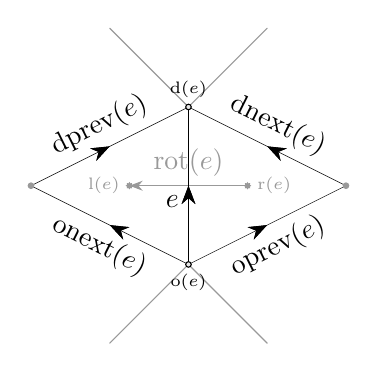
\begin{tikzpicture}[
  line/.style = {thin, color=accent},
  point/.style = {accent},
  face/.style={star, star points = 8, accent},
  arrowmark/.style = {
    postaction=decorate,
    decoration={
        markings,
        mark=at position .5 with {\arrow[thick]{#1}}
    }
  },
  >={Stealth[scale = 1.0]},
]

  %\tkzDefPoint(-0.5,0.0){min}
  %\tkzDefPoint(2.5,3.0){max}

  \tkzDefPoint(0.0,0.0){v0}
  \tkzDefPoint(0.0,2.0){v1}

  \tkzDefPoint(-2.0,1.0){v2}
  \tkzDefPoint(2.0,1.0){v3}

  \tkzDefPoint(-1.0,-1.0){v4}
  \tkzDefPoint(1.0,-1.0){v5}

  \tkzDefPoint(-1.0,3.0){v6}
  \tkzDefPoint(1.0,3.0){v7}

  %\tkzDrawSegments(v0,v1)

  %\tkzDrawSegments[line](v0,v2 v1,v3)
  %\tkzDrawSegments[line](v0,v3 v2,v1)
  \tkzDrawSegments[line](v4,v0 v0,v5)
  \tkzDrawSegments[line](v6,v1 v1,v7)

  \tkzCircumCenter(v0,v1,v2)\tkzGetPoint{f0}
  \tkzCircumCenter(v0,v1,v3)\tkzGetPoint{f1}
  \tkzDrawSegment[line,<-](f0,f1)
  \tkzLabelSegment[above,accent](f0,f1){$\mathrm{rot}(e)$}


  \tkzDrawSegments[arrowmark=Stealth](v0,v1 v0,v2 v0,v3 v2,v1 v3,v1)
  %\tkzMarkSegments[arrowmark=Stealth](v0,v1)
  \tkzLabelSegment[below left](v0,v1){$e$}
  \tkzLabelSegment[sloped,below](v0,v2){$\mathrm{onext}(e)$}
  \tkzLabelSegment[sloped,below](v0,v3){$\mathrm{oprev}(e)$}
  \tkzLabelSegment[sloped,above](v2,v1){$\mathrm{dprev}(e)$}
  \tkzLabelSegment[sloped,above](v3,v1){$\mathrm{dnext}(e)$}

  \tkzDrawPoints(v0,v1)
  \tkzDrawPoints[point](v2,v3)
  \tkzLabelPoint[below](v0){\fontsize{6}{8}\selectfont $\mathrm{o}(e)$}
  \tkzLabelPoint[above](v1){\fontsize{6}{8}\selectfont $\mathrm{d}(e)$}
  \tkzDrawPoints[face](f0,f1)
  \tkzLabelPoint[left,accent](f0){\fontsize{6}{8}\selectfont $\mathrm{l}(e)$}
  \tkzLabelPoint[right,accent](f1){\fontsize{6}{8}\selectfont $\mathrm{r}(e)$}
  % \tkzLabelPoints(v0,v1,v2,v3,v4,v5,v6,v7)


\end{tikzpicture}
\end{document}
